% !TEX root = ../proj_report_outline.tex
\chapter{Additional Proofs}
\begin{prop} [Identity Tensor] \label{prop:identity}
	\(\tensor{H} \in \mathbb{R}^{N \times N \times N}\) such that
\begin{align}
\vec{x}^\mathsf{T}\tensor{H}\vec{y} = \vec{x} \odot \vec{y}, 
&&\forall \vec{x},\vec{y} \in \mathbb{R}^{N}
\end{align} implies
\begin{equation}
	H_{ijk} = \begin{cases}
		1 & \text{if}\;\;i = j = k \\
		0 & \text{otherwise.}
	\end{cases}
\end{equation}

\end{prop}
\begin{proof}
We prove briefly, by inspecting one component of the result. Let 
\(\vec{z} = \vec{x}^\mathsf{T}\tensor{H}\vec{y}\). Then
\begin{align}
	z_j &= \vec{x}^\mathsf{T}\mat{H}_{\midbullet j \midbullet}\vec{y} \\
		&= \sum_i^N\sum_k^N x_iH_{ijk}y_k
\end{align}
If \(z_j = x_jy_j\) as in the elementwise product, then it is clear we want \(H_{ijk}\) to be 
1 if \(i=j=k\). Further, if we ensure \(H_{ijk}\) is 0 when this is not the case we can see that
the rest of the terms in the sums will disappear.
\end{proof}

\chapter{Initialization}
RNNs can be quite sensitive to initialisation, especially with regard to learning long
time dependencies \autocite{Le2015}. It has been suggested that a good initialisation should
have eigenvalues on or inside the complex unit circle \autocite{Zilly2016, Mikolov2015} which
would suggest initialising to an orthogonal or orthonormal matrix as per \autocite{Henaff2016}.

Figure~\ref{fig:inits} shows some simplified simulation to illustrate the effect of
different methods of initialisation with different forms of gated recurrence. They are
simulated with no non-linearity and a single input at the first time step sampled from a unit
normal. If gate values are required, they are sampled uniformly in \([0,1]\). We then simply
run the recurrence over the hidden state for a number of time steps plotting each cell's state
as a grayscale value.

We show three possible procedures: random normal (mean 0, standard deviation 0.01), spectral
normalised and orthonormal. The spectral normalised matrix is a random normal matrix that
has been divided by a fraction of its leading singular value. This ensures the spectral
radius of the matrix is slightly greater than one. To generate a random orthonormal matrix
we generate a random matrix from a normal distribution, compute its QR decomposition and use the
Q.

\begin{figure}
\centering
\begin{subfigure}[t]{0.3\textwidth}

\includegraphics[width=\textwidth]{appendix/init/vanillanormal}
\caption{Vanilla transition, normal initialisation.}
\end{subfigure}~
\begin{subfigure}[t]{0.3\textwidth}
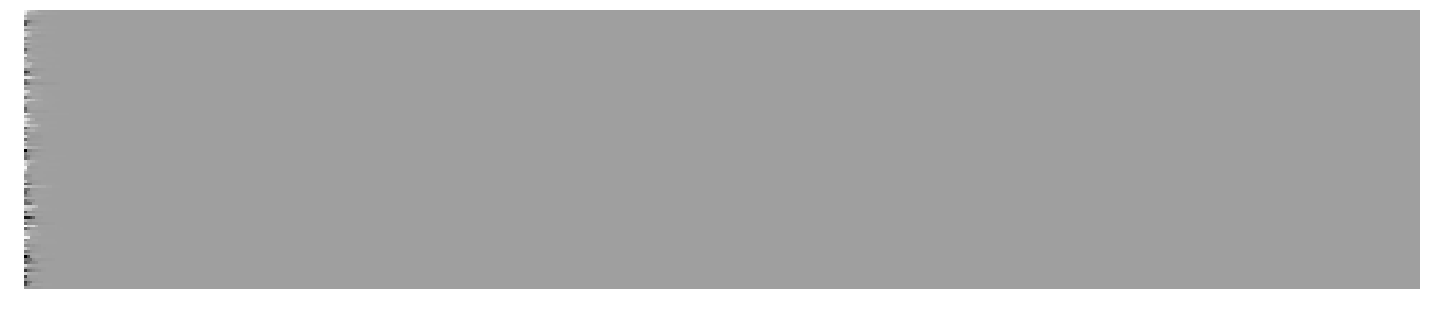
\includegraphics[width=\textwidth]{appendix/init/lstmnormal}
\caption{Forget gate transition, normal initialisation.}
\end{subfigure}~
\begin{subfigure}[t]{0.3\textwidth}
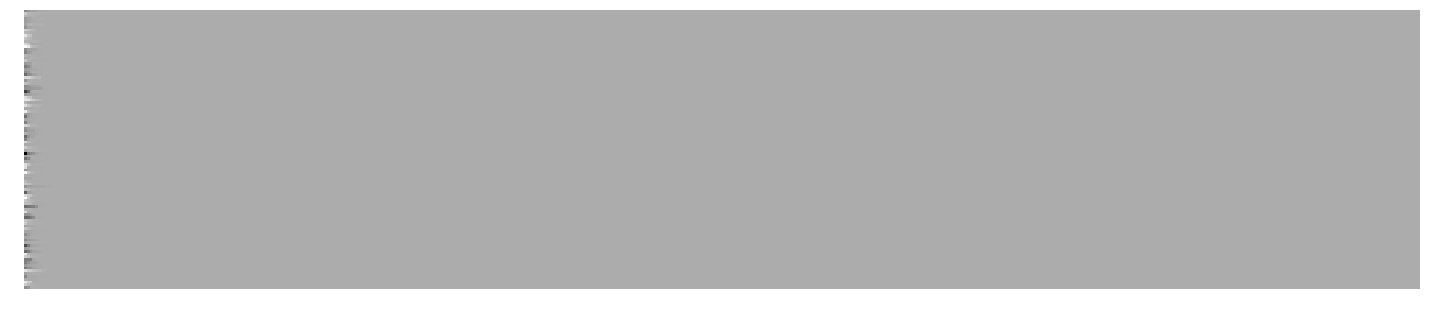
\includegraphics[width=\textwidth]{appendix/init/grunormal}
\caption{Convex gate transition, normal initialisation.}
\end{subfigure}\\

\begin{subfigure}[t]{0.3\textwidth}
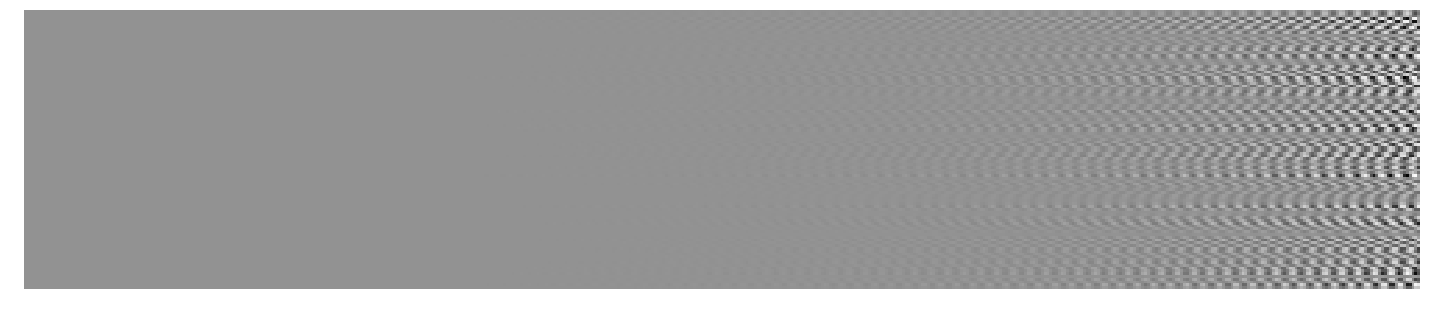
\includegraphics[width=\textwidth]{appendix/init/vanillaspec}
\caption{Vanilla transition, spectral normalised initialisation.}
\end{subfigure}~
\begin{subfigure}[t]{0.3\textwidth}

\includegraphics[width=\textwidth]{appendix/init/lstmspec}
\caption{Forget gate transition, spectral normalised initialisation.}
\end{subfigure}~
\begin{subfigure}[t]{0.3\textwidth}
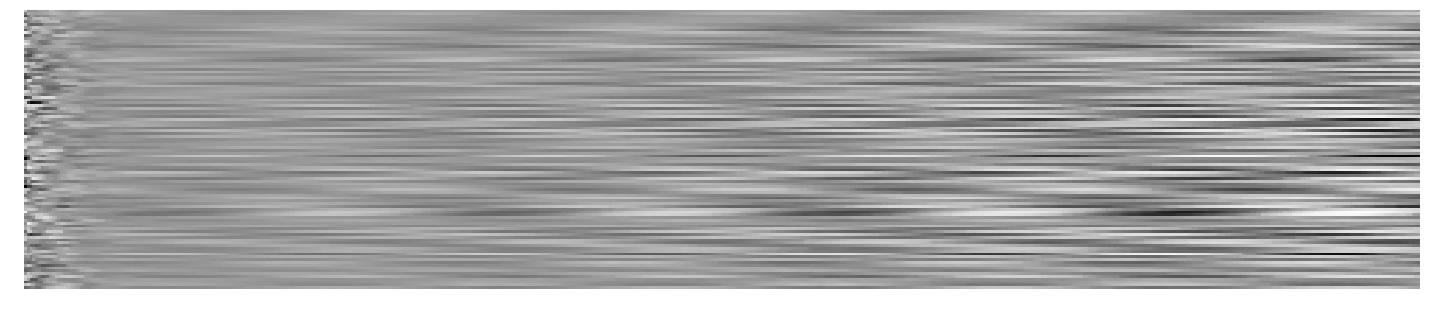
\includegraphics[width=\textwidth]{appendix/init/gruspec}
\caption{Convex gate transition, spectral normalised initialisation.}
\end{subfigure}\\

\begin{subfigure}[t]{0.3\textwidth}

\includegraphics[width=\textwidth]{appendix/init/vanillaorth}
\caption{Vanilla transition, orthonormal initialisation.}
\end{subfigure}~
\begin{subfigure}[t]{0.3\textwidth}

\includegraphics[width=\textwidth]{appendix/init/lstmorth}
\caption{Forget gate transition, orthonormal initialisation.}
\end{subfigure}~
\begin{subfigure}[t]{0.3\textwidth}
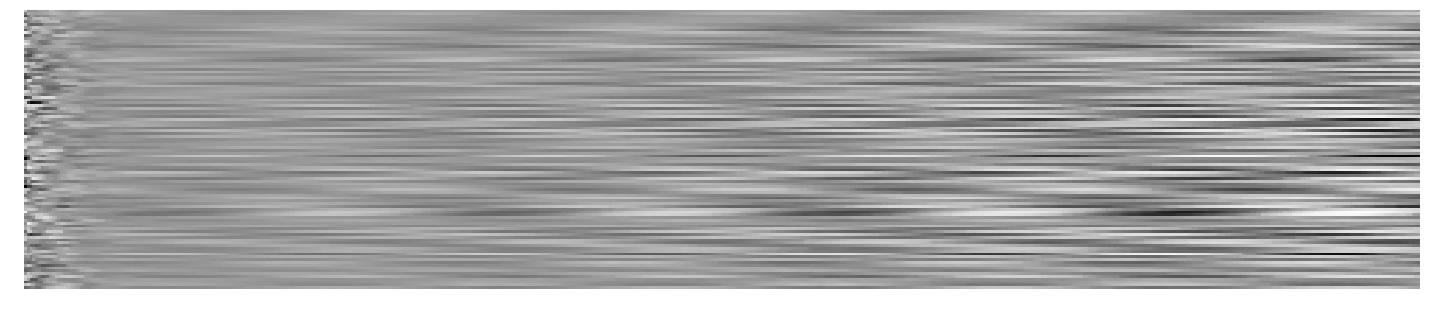
\includegraphics[width=\textwidth]{appendix/init/gruspec}
\caption{Convex gate transition, orthonormal initialisation.}
\end{subfigure}\\

\caption{Example simulations of RNN states from different initialisation. Images are
independently normalised, with darker values being more negative and lighter more positive.}
\label{fig:inits}
\end{figure}

Results are in figure~\ref{fig:inits}. Clearly initialising from a normal distribution is
insufficient. The spectral normalisation also tends to explode (note that often the initial
random state is no longer visible, this is because the degree of normalisation required
to display the final states). Correspondingly we prefer the orthonormal initialisation
throughout this report, although we note that with Vanilla RNNs which preserve information
nearly perfectly from this initialisation we occasionally had to scale the entire matrix down
by a constant factor to avoid exploding early in training.


\chapter{Algorithms for Synthetic Tasks}

\section{Addition}\label{sec:additionpseudo}
Data for the addition task can be generated by algorithm~\ref{alg:additiondata}. This algorithm
produces a single item, it could also be done in batches with slight adjustments.

\begin{algorithm}
	\KwIn{Integer \(T\)}
	\KwOut{Problem instance \((\vec{x}_1, \vec{x}_2, \ldots, \vec{x}_T), y\)}
	\BlankLine
	Sample integer \(i \sim U[1, (T/2)-1]\)\;
	Sample integer \(j \sim U[T/2, T]\)\;
	\(y \gets 0\)\;
	\For{\(t \in \{1, \ldots, T\}\)}{
		Sample float \(x_{t1} \sim U[0,1]\)\;
		\If{\(t = i\) or \(t = j\)} {
			\(y \gets y + x_{t1}\)\;
			\(x_{t2} \gets 1\)\;
		} \Else {
			\(x_{t2} \gets 0\)\;
		}
	}
	\KwRet{\((\vec{x}_1, \vec{x}_2, \ldots, \vec{x}_T), y\)}
	\caption{Generating data for addition task}
	\label{alg:additiondata}
\end{algorithm}

\section{Variable binding}\label{sec:vbindpseudo}
Algorithm~\ref{alg:vbinddata} shows how to generate a single data item for this task. This algorithm
is indicative only, there are ways to be more efficient especially if it has to be implemented as a
computation graph, for example in Tensorflow.

\begin{algorithm}
	\KwIn{Integers \(T, D, N\)}
	\KwOut{Problem instance \((\vec{x}_1,\ldots,\vec{x}_T), (\vec{y}_1,\ldots,\vec{y}_T)\)}
	\BlankLine
	intialise \((\vec{x}_1,\ldots,\vec{x}_T), (\vec{y}_1,\ldots,\vec{y}_T)\) to zeros\;
	\For{\(i \in \{1, \ldots, N\}\)} {
		Sample integer \(j \sim U[1, (T/2)-1]\) \tcc*{start position}
		Sample integer \(k \sim U[j+1, T]\) \tcc*{end position}
		\(\vec{z} \gets\) random \(D\) bit binary pattern\;
		\(\vec{y}_{k+1} \gets \vec{z}\)\;
		Set first \(D\) bits of \(\vec{x}_{i+1}\) to \(\vec{z}\)\;
		\For(set label bits){\(l \in \{j,\ldots,k\}\)}{
			\({x}_{l, D+i} \gets 1\)\;
		}
	}
	\KwRet{\((\vec{x}_1,\ldots,\vec{x}_T), (\vec{y}_1,\ldots,\vec{y}_T)\)}
	
	\caption{Generating data for variable binding}
	\label{alg:vbinddata}
\end{algorithm}